\chapter{Evaluation and comparison}
\emph{%
This chapter begins with the introduction of the used evaluation measurements including a comparison of their strengths and weaknesses based on artificial datasets. Then a recap of all used parameters for DBSCAN and the distance metrics are given. This is followed by the description of the datasets used for the overview of the good and the bad of the two distance metrics, which concludes this chapter.
}\label{chap:eval}

\section{Evaluation measures}\label{sec:cqm}
Cross validation\cite{Park2009} is a common evaluation technique  of probabilistic models as seen in some related works\cite{Hong2012, Yin2011}. There are many different ways to cross validate, but the general idea stays the same: generate the model based on based on a part of the dataset (model set), and evaluate with another (test set), for example with perplexity, or by measuring the average error between predicted location and real location. This is usually done to ensure that the generated model is able to classify previously unknown documents respectively that the model is not to specific to the documents used for generation.

This form of evaluation can hardly be applied to clustering tasks, because their is no standard way to classify unknown, unused objects to an existing clustering; other than to cluster the data again. Therefore there are other evaluation measures, which could also be used with probability models. Clustering evaluation measures try to measure the goodness of a clustering. Because the \enquote{goodness} is usually domain and task dependent, there are many different cluster quality measures (CQM).

%external
A rough classification of the different quality evaluation measures would group them into either \emph{external} or \emph{internal} quality measures\cite{Rendon2011}. External indices use domain or a priori knowledge. The two popular external measures \emph{precision} and \emph{recall} for example are using existing and correct classification information of datasets (also called gold standards) and are calculated by using the number of items correctly (or falsely) labelled. 
%f-scan

%internal
Internal evaluation measures only use the information provided by the dataset itself. This boils mostly down to using either the \emph{compactness} or the \emph{separability} of the resulting clustering, or both.
%
Compactness measures the closeness of elements in a cluster, while separability indicates how distinct two clusters are by computing the distance between two different clusters.

Datasets containing a priori knowledge usable for external evaluation measures are generally either artificial or hand annotated; meaning that most real problems and natural datasets contain no external knowledge for external evaluation measures.  Therefore the following indices used in this thesis are all internal evaluation measures.
%\newpage

\subsection{Dunn index}
The Dunn index\cite{Dunn1973} $D$ defines the ratio between the minimal inter cluster distance to the maximal intra cluster distance.

\begin{align}
D = \frac{d_{min}}{d_{max}},
\end{align}
%
where $d_{min}$ denotes the smallest distance between two objects from different clusters, and $d_{max}$ the largest distance of two objects from the same cluster.

\vspace{.5em}
\noindent
The Dunn index is limited to the interval $[0, \infty]$ and should be maximized.


\subsection{Davies-Bouldin index}
The Davies-Bouldin index\cite{Davies1979} $DB$ is defined as:

\begin{align}
DB = \frac{1}{n} \sum^n_{i=1, i \neq j} max(\frac{\rho_i + \rho_j}{d(center_i, center_j)})
\end{align}
%
where $n$ is the number of clusters, $\rho_i$ is the average distance of all documents in cluster $c_i$ to their cluster center $center_i$ and $d(center_i, center_j)$ is the distance of the two cluster centers $center_i$ and $center_j$. Small values of $DB$ correspond to clusters that are compact, and whose cluster centers are far away from each other.

\vspace{.5em}
\noindent
The Davies-Bouldin index is limited to the interval $[0, \infty]$ and should be minimized.

\subsection{C-index}
The C-index\cite{Hubert1976} $C$ is defined as:
\begin{align}
C = \frac{S - S_{min}}{S_{max} - S_{min}},
\end{align}
%
where $S$ is the sum of distances over all pairs of objects from the same cluster, $n$ is the number of those pairs and $S_{min}$ is the sum of the $n$ smallest distances if all pairs of objects are considered. Likewise $S_{max}$ is the sum of the $n$ largest distances out of all pairs.

\vspace{.5em}
\noindent
The C-index is limited to the interval $[0, 1]$ and should be minimized.


%Boros-Clustering-2011-May-24
\subsection{Silhouette width}
The silhouette width\cite{Rousseeuw1987} $SW_i$ indicates how well element $i$ was clustered.

\begin{align}
SW_i = \frac{b_i-a_i}{max(a_i, b_i)},
\end{align}
where $a_i$ is the average distance from point $p_i$ to all other points in his cluster, and $b_i$ is the minimum average distance from point $p_i$ to all points in the another clusters. The average silhouette width $ASW$ then measures the global goodness of a clustering.

\begin{align}
ASW = \frac{\sum_i SW_i}{n}
\end{align}

\vspace{.5em}
\noindent
The average silhouette width is limited to the interval $[-1, 1]$ and should be maximized.

\subsection{Quality check}\label{sec:qcheck}
Unfortunately these quality measures have their strengths and weaknesses. Those will be explored based on artificial datasets. These CQMs are useful at comparing different clusterings, but can they also be used to indicate a global goodness?

Figure~\ref{fig:clusterexamples} shows four synthetic point arrangements coloured after their cluster categorisation, while table~\ref{tbl:syn_compare} lists the respective measurement scores.
\begin{description}
\item[blobs] shows three clearly distinguishable point clusters
\item[random] shows points randomly distributed in space; the clustering is also random in this case
\item[moons] shows two half-moon shaped point arrangements
\item[circles] shows two rings, a small one inside a bigger one
\end{description}

\begin{figure}%[hbt]
\centering	
	\begin{subfigure}[b]{0.22\textwidth}
		\centering
		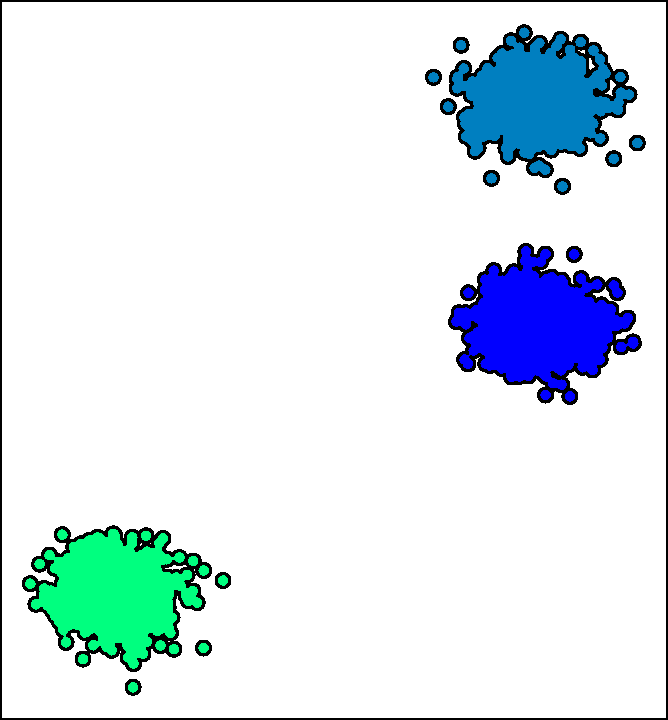
\includegraphics[height=\textwidth]{pix/blobs_color_3600.pdf}
		\caption{blobs}
	\end{subfigure}
	\hspace*{0.01\textwidth}	
	\begin{subfigure}[b]{0.22\textwidth}
		\centering
		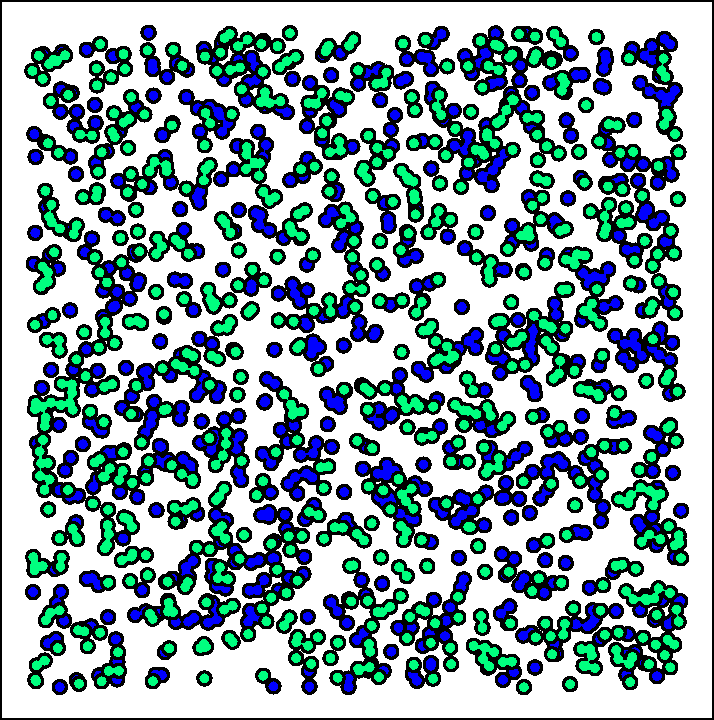
\includegraphics[height=\textwidth]{pix/random_color_3600.pdf}
		\caption{random}
	\end{subfigure}
	\hspace*{0.015\textwidth}	
	\begin{subfigure}[b]{0.22\textwidth}
		\centering
		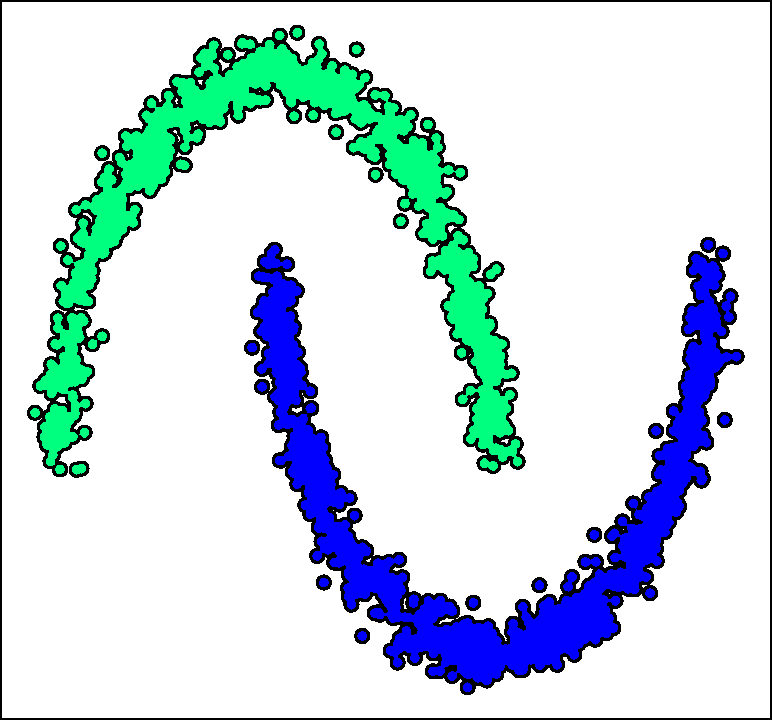
\includegraphics[height=\textwidth]{pix/noisy_moons_color_3600.pdf}
		\caption{moons}
	\end{subfigure}
	\hspace*{0.035\textwidth}	
	\begin{subfigure}[b]{0.22\textwidth}
		\centering
		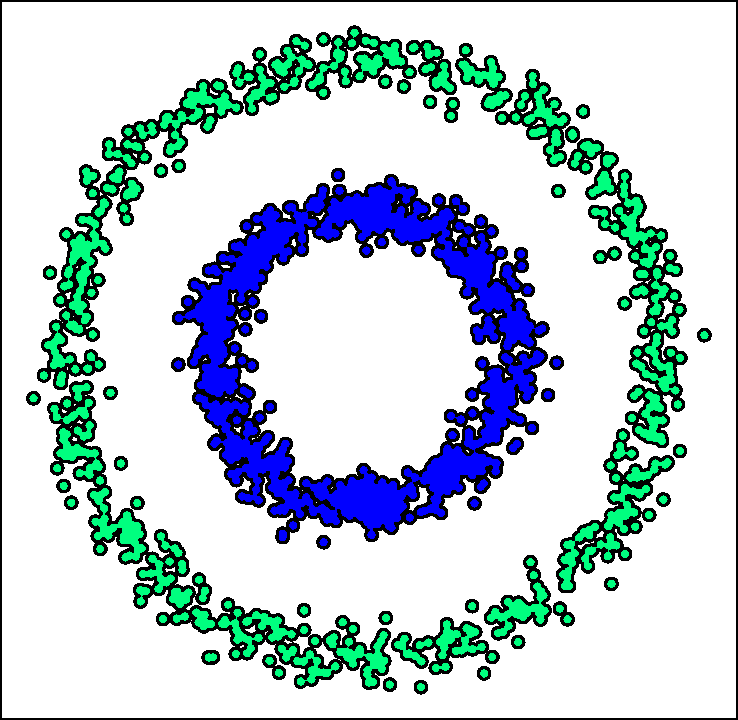
\includegraphics[height=\textwidth]{pix/noisy_circles_color_3600.pdf}
		\caption{circles}
	\end{subfigure}    
\caption{Synthetic clustering examples}\label{fig:clusterexamples}
\end{figure}
%\begin{figure}[Hht]
%\centering
%	\begin{subfigure}[b]{0.3\textwidth}
%		\centering
%		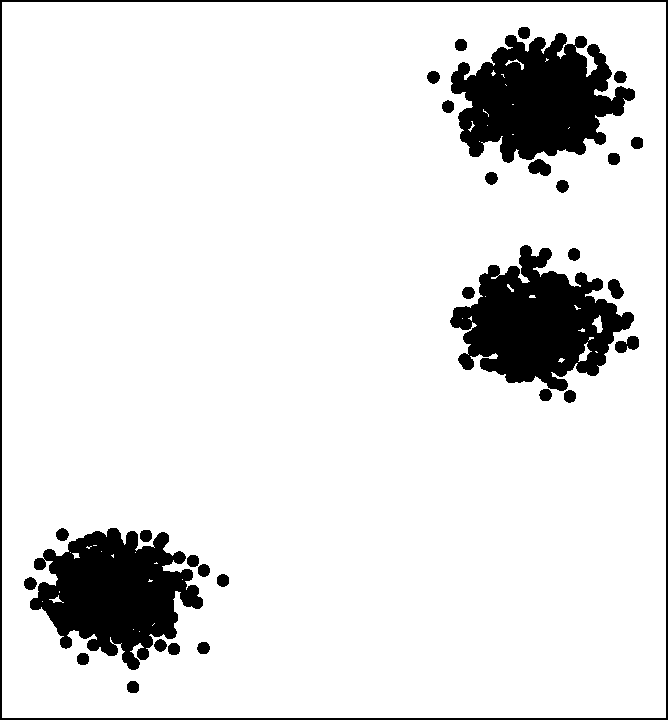
\includegraphics[width=\textwidth]{pix/blobs_scatter.pdf}
%		%\caption{Blobs}
%		%\label{fig:gull}
%	\end{subfigure}
%	\,
%	\begin{subfigure}[b]{0.3\textwidth}
%		\centering
%		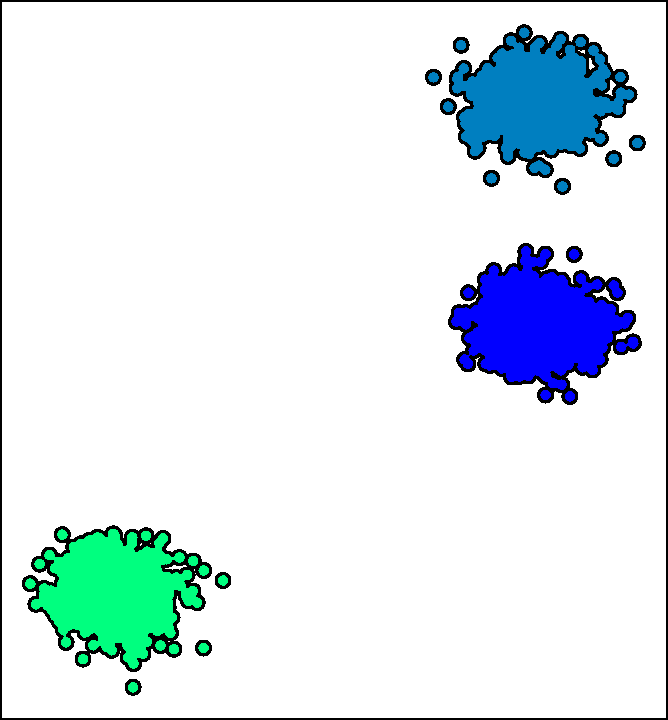
\includegraphics[width=\textwidth]{pix/blobs_color_3600.pdf}
%		%\caption{Random}
%		%\label{fig:gull}
%	\end{subfigure}
%	
%	\hfill
%	
%	\begin{subfigure}[b]{0.3\textwidth}
%		\centering
%		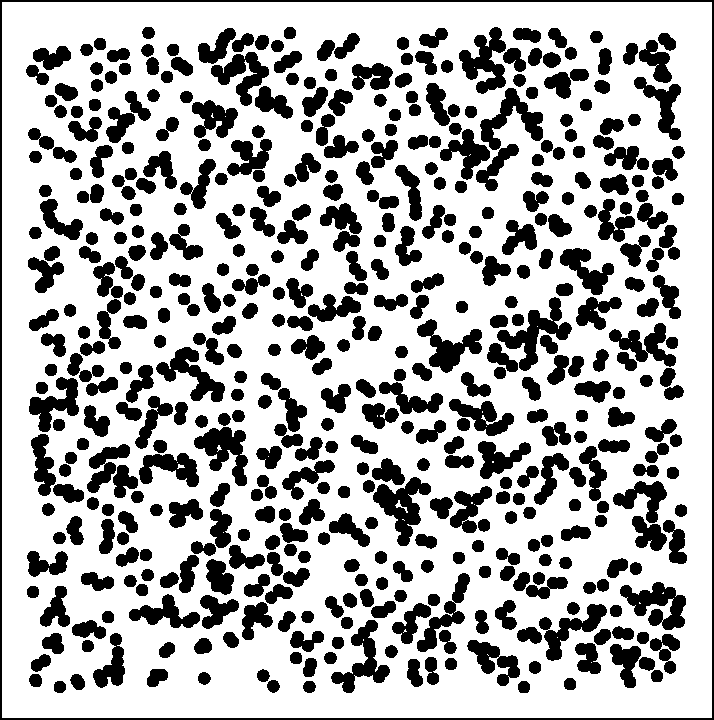
\includegraphics[width=\textwidth]{pix/random_scatter.pdf}
%		%\caption{Random}
%		%\label{fig:gull}
%	\end{subfigure}
%	\,
%	\begin{subfigure}[b]{0.3\textwidth}
%		\centering
%		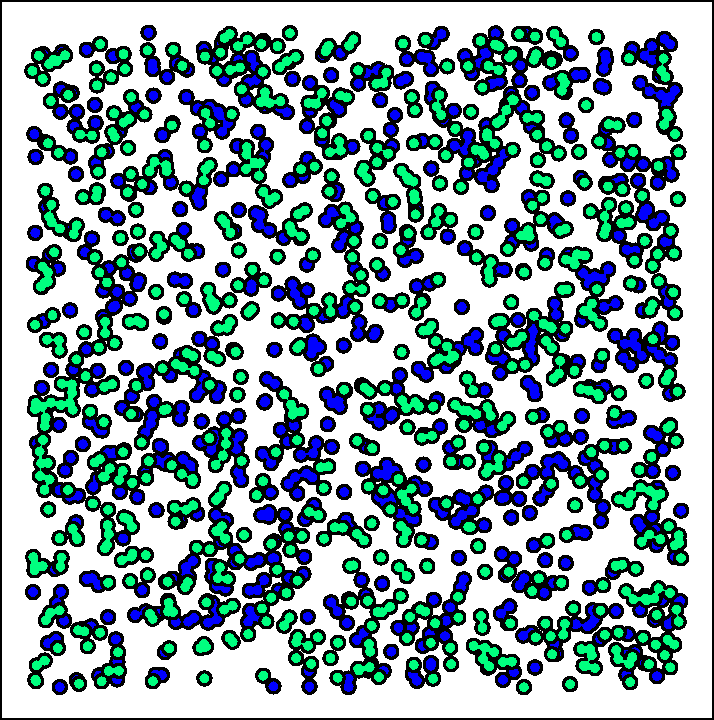
\includegraphics[width=\textwidth]{pix/random_color_3600.pdf}
%		%\caption{A gull}
%		%\label{fig:gull}
%	\end{subfigure}
%
%	\hfill
%
%	\begin{subfigure}[b]{0.3\textwidth}
%		\centering
%		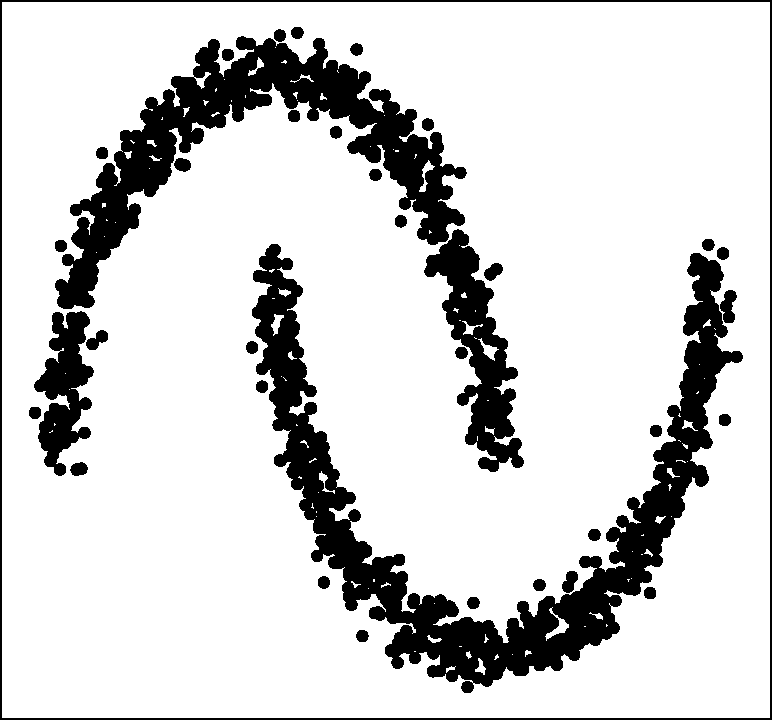
\includegraphics[width=\textwidth]{pix/noisy_moons_scatter.pdf}
%		%\caption{Half-moons}
%		%\label{fig:gull}
%	\end{subfigure}
%	\,
%	\begin{subfigure}[b]{0.3\textwidth}
%		\centering
%		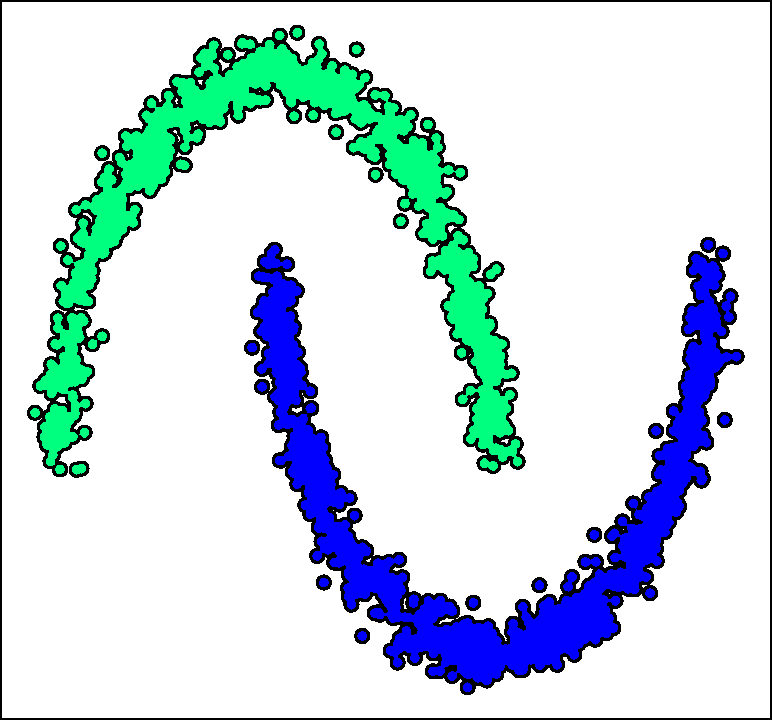
\includegraphics[width=\textwidth]{pix/noisy_moons_color_3600.pdf}
%		%\caption{A gull}
%		%\label{fig:gull}
%	\end{subfigure}
%
%	\hfill
%
%	\begin{subfigure}[b]{0.3\textwidth}
%		\centering
%		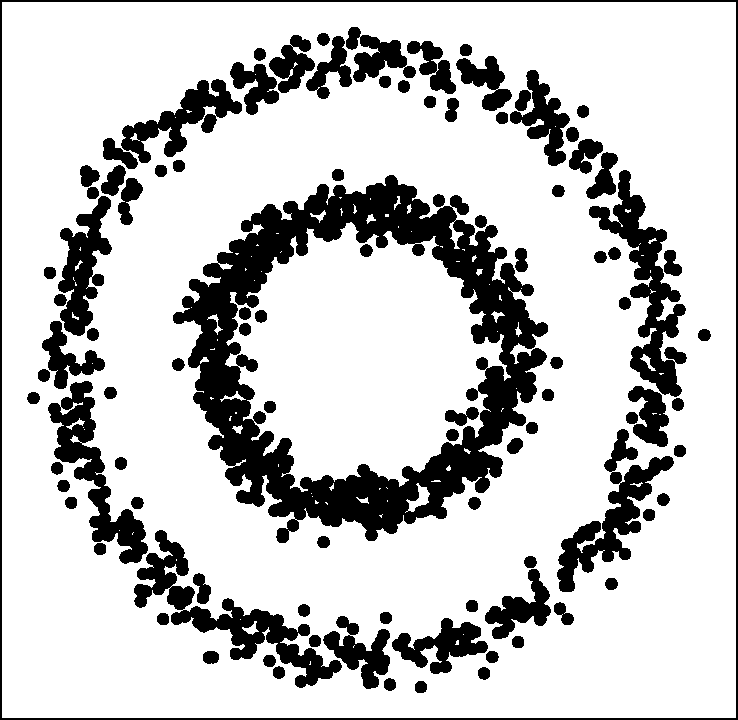
\includegraphics[width=\textwidth]{pix/noisy_circles_scatter.pdf}
%		%\caption{Circles}
%		%\label{fig:gull}
%	\end{subfigure}
%	\,
%	\begin{subfigure}[b]{0.3\textwidth}
%		\centering
%		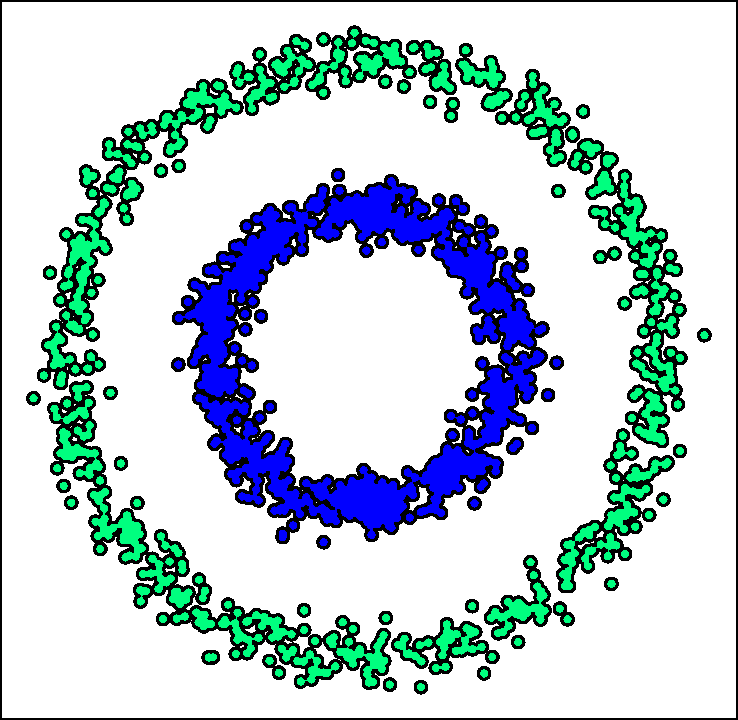
\includegraphics[width=\textwidth]{pix/noisy_circles_color_3600.pdf}
%		%\caption{A gull}
%		%\label{fig:gull}
%	\end{subfigure}        
%\caption{Synthetic clustering examples}\label{fig:clusterexamples}
%\end{figure}

\begin{table}%[bth]
\caption{Comparison of the evaluated synthetic test cases}\label{tbl:syn_compare}
\centering
\sisetup{table-format = 1.0(1)e2}
\begin{tabular}{cSSSS}
\toprule
Dataset & {DB} &{C}&{SW}&{D}\\
			& {\scriptsize $0<min<\infty$} &{\scriptsize $0<min<1$}&{\scriptsize $-1<max<1$}&{\scriptsize $0<max<\infty$}\\
\midrule
blobs	& 1.35e-02 & 3.18e-09 & 9.87e-01& 3.13e+00\\
circles	& 1.36e+00& 5.01e-01 & 1.11e-01 & 1.43e-02\\
moons	& 3.31e-01 & 1.50e-01 & 5.25e-01 & 5.01e-02\\
random& 5.29e+01 & 5.00e-01 & 1.91e-03 & 9.67e-07\\
\bottomrule
\end{tabular}
\end{table}
%
\newpage
It is obvious that those clusters are optimal. Sadly every cluster measurement fail in one way or another. Except 
\begin{description}
\item[DB,] which shows a bad result for $random$, and good ones for the others. $circles$ is here a little worse than $blobs$ and $moons$, because its two cluster centers are very close to each other.

\item[C] indicates a good results for $blobs$ and $moons$, but regards $circles$ and $random$ equally mediocre, but nor really bad either. It seems they both share the same ratios of minimum to maximum distances and their respective sums.

\item[SW] performs well for $blobs$ and $moons$. But less well for $circles$---the average distances to the two clusters seem not too be that far apart. The $random$ clustering scores as expected; its average distances should be the same for the two randomized clusters.

\item[D] scores $blobs$ really high, but not the rest. Big or widespread clusters have higher maximum distances. When those clusters are fairly near together, their score drops significantly.
\end{description}
%
After this short test comparison, it should be clear to not trust those scores blindly. A few more aspects of how a good clustering should look are now presented. These are very subjective aspects, and will differ from case to case. But they help to address different points of views and to discuss those, if needed.
%
\begin{description}
\item[Noise] The amount of documents regarded as $noise$ should not be high. There could always be documents which do not fit to the available clusters, but $noise$ should be minimized, either through better distance functions or a better dataset. $noise$-threshold in this thesis is set to the arbitrary amount of maximal a quarter of the dataset size.
\item[Number of clusters] Some algorithms, like k-means, need this as a parameter. A common approach is to use a CQM and take the amount of clusters which maximises the score. This can work, if the CQM is carefully chosen. Arbitrary baseline is, that there should be 2 order of magnitudes between the size of the dataset and the number of clusters.
\item[Items per cluster] The distribution of items per cluster is also to take into account. The best case is an even distribution (every cluster has the same size). But this is unfortunately never the case. A power-law distribution is more common, where the most documents are clustered in a very few clusters.
\end{description}
%
The search for good clusters is after all very subjective and depended on domain knowledge. But rules for filtering the worst results on the considerations above are easy to write.

\section{Parameter choice}
The choice of the parameters used for creating the clusterings that are going to be compared is very crucial. To present a clear picture about the possibilities of the evaluated algorithms, or distance metrics, the parameters delivering the best results should be always used. But finding these parameters in a reasonable time is not always possible. 

Because of that, the time and effort of finding good setting should either be quantitatively reflected in the final verdict, or be equally distributed between the candidates. The later is usually done, by using domain knowledge and common sense for the parameter choice.

Presented now is a recap of all the available parameters which have influence on the cluster results and explanations for the values used.

DBSCAN has the two parameters $eps$ and $minPts$, which describe how much points ($minPts$) have to be at least in an $eps$-neighbourhood of a point for it to be considered dense and part of a cluster. The usual approach is to lock $minPts$ and experiment with $eps$.
%
\begin{align*}
minPts &= 4 & eps_{DBSCAN} &= \dots\\
\intertext{The combined distance has weight and threshold parameters for normalising the distances. The idea behind the normalization is, to get exactly $1.0$ if both distances are equal to their thresholds. Therefore $eps_{DBSCAN}$ is set to $1.0$. Weights and thresholds are both multiplied with each other, so we lock the weights to $0.5$ and experiment with the thresholds.}
eps_{DBSCAN} &= 1.0\\
w_{text} &= 0.5	&	w_{location} &= 0.5\\
eps_{text} &= [0.1, 0.5, 0.9] & eps_{location} &= \dots\\
\intertext{The random walk distance has parameter controlling the generation and weights of the graph. Here is no easy normalisation scheme, thus $eps_{DBSCAN}$ is used as intended for experimentation. The weights of the attributes are relative to each other, therefore $w_{location}=1.0$, while $w_{text}$ is set to different values. Edges which are too long can be removed from the graph based $km$. This value is based on the visual impression regarding the overall distribution of short and long edges; visualisations can be seen in figures~\ref{fig:A}, \ref{fig:B} and \ref{fig:C}. Finally there is $c=0.1$ and $l=20$. $c$ is the restart probability and $l$ the length of the random walk. Both are set as described in \cite{Zhou2009}.}
eps_{DBSCAN} &= \dots & km &= \text{based on visual impression}\\
c &= 0.1 & l &= 20\\
w_{text} &= [0.1, 1.0, 2.0] & w_{location} &= 1.0
\end{align*}
%
The search ranges (noted above as $\dots$) are manually explored with the settings above, based on the considerations from the previous section~\ref{sec:qcheck}. The best looking findings are then quantitatively measured with the described CQMs.

\section{Datasets}\label{sec:datasets}
For the comparison between the two approaches three datasets have been used. Table~\ref{tbl:datasets} shows the details. It can be seen that dataset A from Twitter has much more different words and points than B and C from Flickr, especially when considering the document size. This could result from the different usages of the services. Twitter user are much more mobile, and usually do not sent many tweets from the same location, while Flickr photos, when taken from the same spot, or geotagged afterwards, have much more locations in common. This results in a general different distribution of points in space and the generated graphs are much more sparse for B and C, as seen in figures~\ref{fig:A}, \ref{fig:B} and \ref{fig:C}. Dataset C was also used by \textcite{Sengstock2012a}.

The used words are also very different. While Flickr tags are more descriptive, Twitter tweets have much more abbreviated and strange words, due to the limitation on 140 characters per tweet. The usage again leads to very different characteristics as seen in table~\ref{tbl:top_words}. Datasets B and C have easy to recognise words, while A contains even numbers in its top ten of words. Word distributions are also very different. Having a few words with high count in contrast to the majority with low count is usual. This can be seen in B and C, where the tenth has approximately half the count of the first, but the distribution of A is very distorted, with the first having eight times the count of the tenth word. 

\begin{table}
\caption{Details of the datasets}\label{tbl:datasets}
\centering
\begin{tabular}{crrrcc}
\toprule
Dataset	& \# documents & \# unique points & \# words&source&general location\\
\midrule
A	& \num{57554}	&	\num{25665} & \num{30001}	&Twitter&Germany\\%Dataset Germany small
B	& \num{1254298}	&	\num{8831} & \num{3229} &Flickr&Germany\\%Dataset Germany
C	& \num{1086678}	&	\num{12992} & \num{4373} &Flickr&United States\\%Dataset USA small 1M
\bottomrule
\end{tabular}
\end{table}



%\afterpage{
\begin{figure}[p]
	\begin{subfigure}[b]{0.49\textwidth}
	\centering
	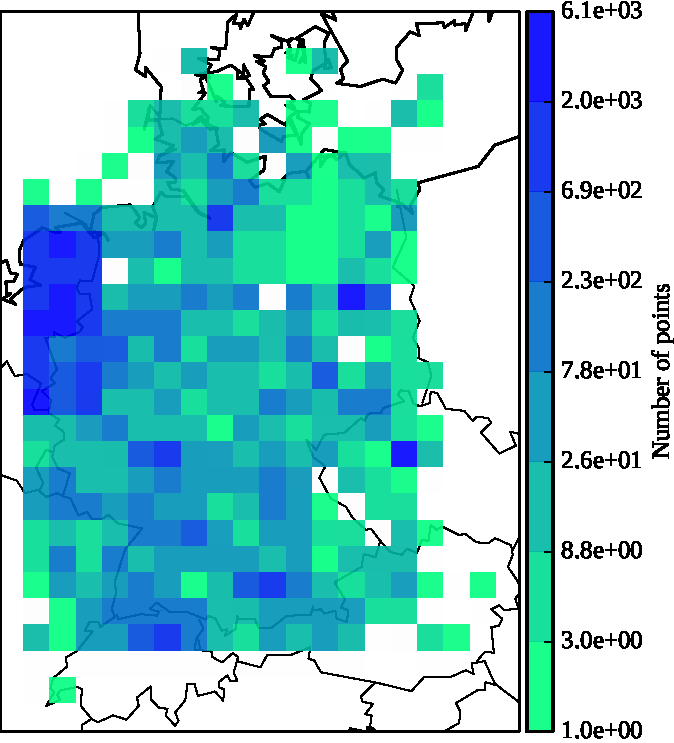
\includegraphics[width=.99\textwidth]{pix/freq_ger_small.pdf}
		\caption{Frequency plot}
		%\label{fig:gull}
	\end{subfigure}
	%
	\begin{subfigure}[b]{0.482\textwidth}
	\centering
	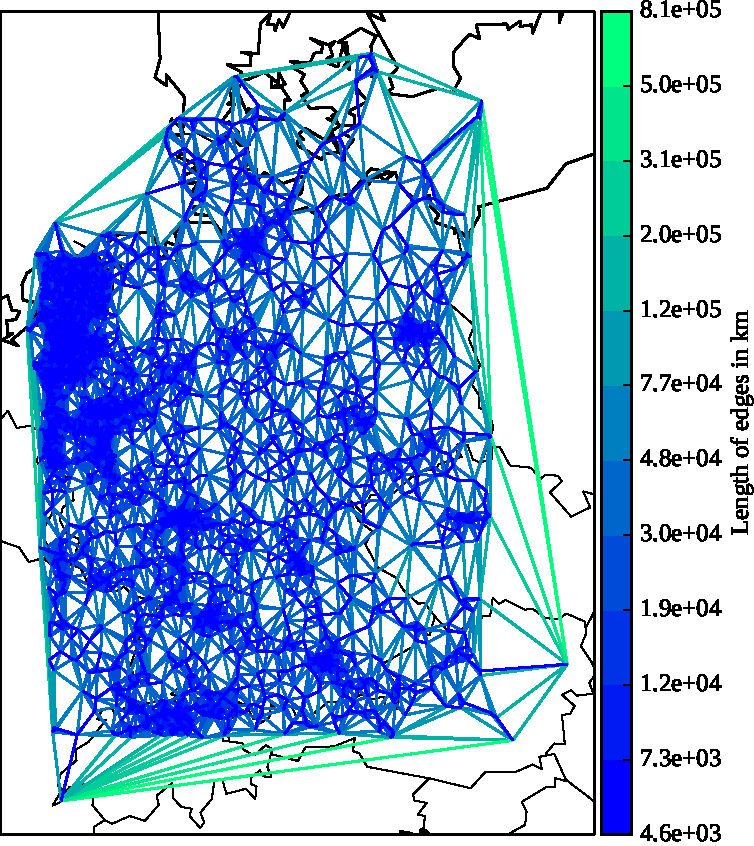
\includegraphics[width=.99\textwidth]{pix/tri_ger_small.pdf}
		\caption{Edge plot}
		%\label{fig:gull}
	\end{subfigure}
	\caption[Dataset A frequency and edge plots]{Dataset A pictures}
	\label{fig:A}
\end{figure}
%
\begin{figure}[p]
	\begin{subfigure}[b]{.49\textwidth}
	\centering
	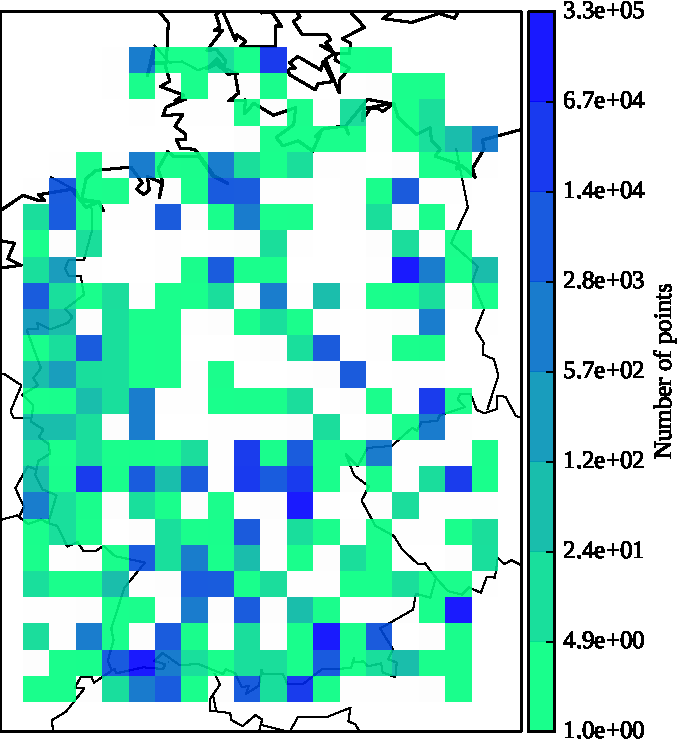
\includegraphics[width=.99\textwidth]{pix/freq_ger.pdf}
		\caption{Frequency plot}
		%\label{fig:gull}
	\end{subfigure}
	%
	\begin{subfigure}[b]{.482\textwidth}
	\centering
	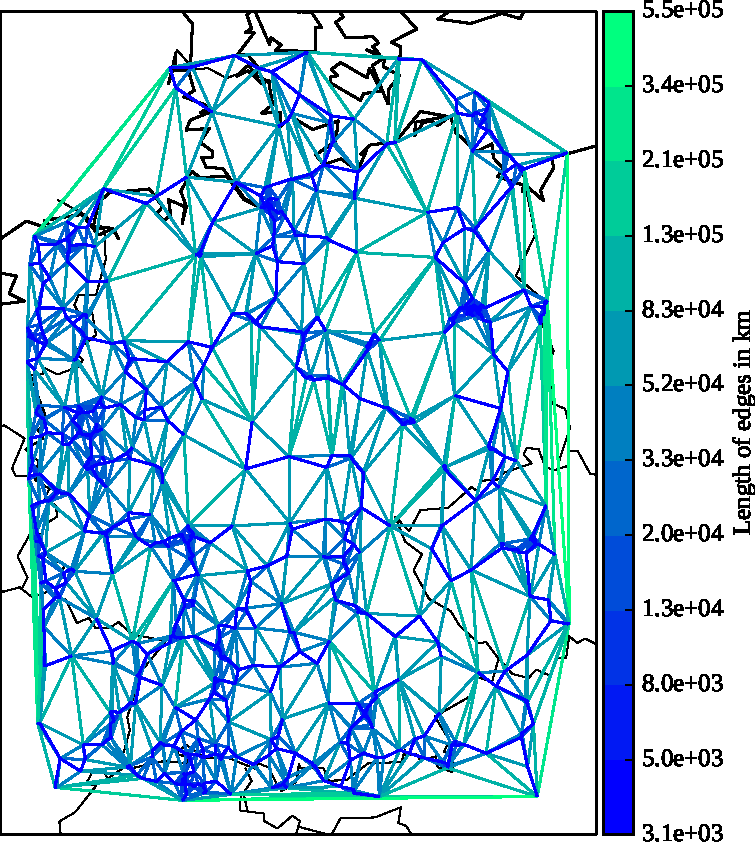
\includegraphics[width=.99\textwidth]{pix/tri_ger.pdf}
		\caption{Edge plot}
		%\label{fig:gull}
	\end{subfigure}
	\caption[Dataset B frequency and edge plots]{Dataset B pictures}
	\label{fig:B}
\end{figure}
%
%\clearpage
%}

%\afterpage{
\begin{figure}[p]
	\begin{subfigure}[b]{\textwidth}
	\centering
	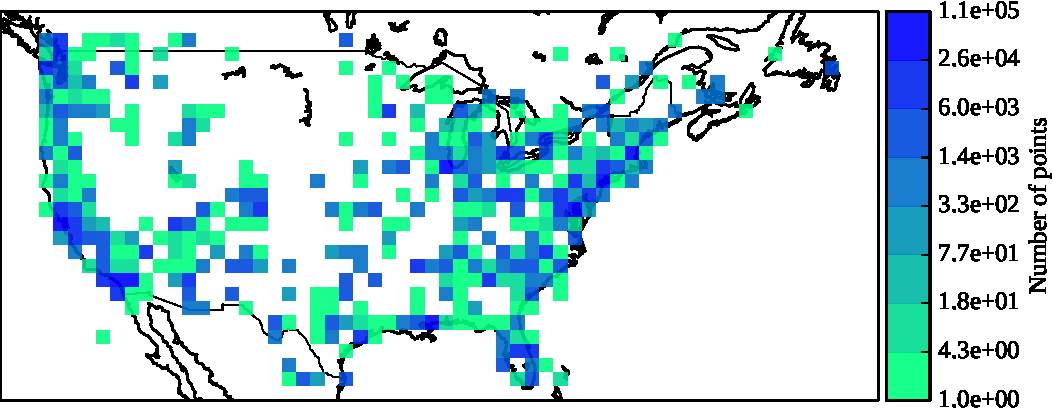
\includegraphics[width=1.\textwidth]{pix/freq_usa_small.pdf}
		\caption{Frequency plot}
		%\label{fig:gull}
	\end{subfigure}
	%
	\begin{subfigure}[b]{\textwidth}
	\centering
	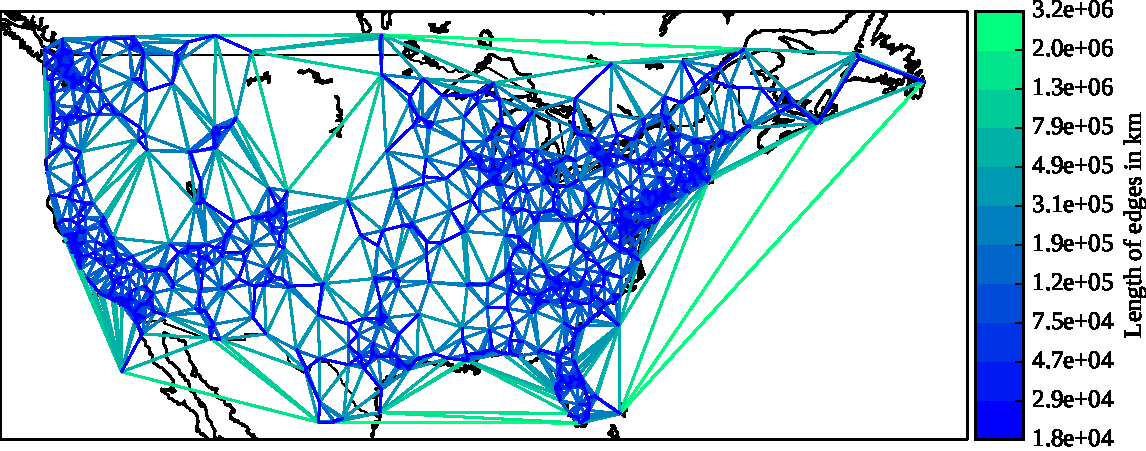
\includegraphics[width=1.\textwidth]{pix/tri_usa_small.pdf}
		\caption{Edge plot}
		%\label{fig:gull}
	\end{subfigure}
	\caption[Dataset C frequency and edge plots]{Dataset C pictures}
	\label{fig:C}
\end{figure}
%\enlargethispage{5\baselineskip}

%\begin{table}[htb]
%\caption{Ten most words in the datasets}
%\footnotesize
%\label{tbl:top_words}
%\begin{subtable}{.33\linewidth}
%\centering
%\begin{tabular}{cr}
%\toprule
%\multicolumn{2}{c}{dataset A}\\
%\midrule
%nowplaying & \num{4494}\\
%acakfilm & \num{4086}\\
%ger & \num{1666}\\
%pp11 & \num{1464}\\
%176 & \num{1242}\\
%brandenburg & \num{1107}\\
%twexit & \num{986}\\
%fb & \num{960}\\
%9748 & \num{728}\\
%bbradio & \num{656}\\
%\bottomrule
%\end{tabular}
%%\caption{A}
%\end{subtable}
%%
%\begin{subtable}{.33\linewidth}
%\centering
%\begin{tabular}{cr}
%\toprule
%\multicolumn{2}{c}{dataset B}\\
%\midrule
%iphoto & \num{185322}\\
%schluchsee & \num{185322}\\
%ostern & \num{178653}\\
%osterbrunnentour & \num{178653}\\
%easter & \num{178652}\\
%germany & \num{177129}\\
%decoration & \num{156301}\\
%dekoration & \num{156296}\\
%ei & \num{156295}\\
%custom & \num{156294}\\
%\bottomrule
%\end{tabular}
%%\caption{B}
%\end{subtable}
%%
%%\vspace{.5em}
%%
%\begin{subtable}{.33\linewidth}
%\centering
%\begin{tabular}{cr}
%\toprule
%\multicolumn{2}{c}{dataset C}\\
%\midrule
%usa & \num{137875}\\
%unitedstates & \num{133614}\\
%events & \num{113506}\\
%family & \num{109931}\\
%jackjules & \num{108666}\\
%daddy & \num{108666}\\
%elementsorganizer & \num{68400}\\
%home45drumhillroad & \num{67314}\\
%harrypotterparty & \num{67035}\\
%california & \num{61710}\\
%\bottomrule
%\end{tabular}
%%\caption{C}
%\end{subtable}
%\end{table}
\begin{table}[htb]
\caption{Ten most words in the datasets}\label{tbl:top_words}
\centering
\footnotesize
\begin{tabular}{crcrcr}
\toprule
\multicolumn{2}{c}{dataset A}&\multicolumn{2}{c}{dataset B}&\multicolumn{2}{c}{dataset C}\\
\midrule
nowplaying & \num{4494} & iphoto & \num{185322} & usa & \num{137875}\\
acakfilm & \num{4086} & schluchsee & \num{185322} & unitedstates & \num{133614}\\
ger & \num{1666} & ostern & \num{178653} & events & \num{113506}\\
pp11 & \num{1464} & osterbrunnentour & \num{178653} & family & \num{109931}\\
176 & \num{1242} & easter & \num{178652} & jackjules & \num{108666}\\
brandenburg & \num{1107} & germany & \num{177129} & daddy & \num{108666}\\
twexit & \num{986} & decoration & \num{156301} & elementsorganizer & \num{68400}\\
fb & \num{960} & dekoration & \num{156296} & home45drumhillroad & \num{67314}\\
9748 & \num{728} & ei & \num{156295} & harrypotterparty & \num{67035}\\
bbradio & \num{656} & custom & \num{156294} & california & \num{61710}\\
\bottomrule
\end{tabular}
\end{table}

%\clearpage
%}

%\section{Sampling}
%Running all CEM requires all inter-cluster distances $inter(k, l) = \{d(i,j) \forall i \in c_k, j \in c_l; k \neq l \}$ and all intra-cluster distances $intra(k) = \{d(i,j) \forall i,j \in c_k, i \neq j \}$ for all clusters $\{c_1, \dots c_n\}$, which informatively results in the calculation of all pairwise distances of the dataset. By doubling the size of a dataset, the pairwise distance calculations would quadruple $\propto$. This is not practical considering dataset size of millions of points (and growing).

%For this reason


\section{Comparison}
All algorithms were programmed in C++, with glue-code in Python were necessary. Matrix multiplication is performed with Eigen\cite{Guennebaud2010} and region queries with FLANN\cite{Muja2009}. The test system uses an Intel Q9400 CPU with 4x2.66~GHz and 4~GB RAM, running under Arch Linux with kernel version 3.12.

Qualitative comparison is done imitating a keyword search. Based on a keyword $k$, a new set of documents $D_k$ is compiled and a heatmap representing the distribution in space is generated, alongside a list of word frequencies. $D_k$ consists of all words $w \in c_i$, where $k \in c_i$. The idea behind this is, that in a meaningful geographical topic clustering, all clusters with $k$ in it should be descriptive, or otherwise topical related regarding $k$; thus $D_k$ should describe $k$. Terms are ordered by their frequency in $D_k$, and the first 25 terms of all discussed search sets are listed at the appendix.
%
Quantitative comparison is done by applying the different CQMs described in section~\ref{sec:cqm} with the two basic distance measures for location distance (euclidean distance) and text distance (jaccard distance). Baseline for the combined metric ($CM$) and graph metric ($GM$) is a random clustering ($R$). $R$ is simply generated by evenly distributing elements into 200 clusters, with a probability of 10\% for skipping an element ( meaning noise is around 10\%).

%                                      A GER SMALL
%
\begin{center}
\captionof{table}{Statistics and used parameters for dataset A}
\small
\sisetup{table-parse-only}
\begin{tabular}{cSSSc}
\toprule
 & {clusters} &{clustered elements}&{noise}&{parameters}\\
\midrule
GM & 2082 & 43175 & 14379&$km=40000$, $w_{text} = 1.0$, $\epsilon = 0.9694$\\
CM & 888 & 52418 & 5136&$eps_{text} = 0.1$, $eps_{loc} = 300$\\
\bottomrule
\end{tabular}
\end{center}
%
Dataset A contains the Twitter data from Germany. The used parameters result in much more clusters with much more noise for $GM$. Despite those advantages for $GM$ (more clusters with less documents usually results in better scores), $CM$ fares better in comparison with the CQM as seen in table~\ref{tbl:A_compare}. Both $GM$ and $CM$ compare better agains the random clustering $R$, but text distance measures are all very narrow. Location distance measures are much better, and both $GM$ and $CM$ fare overall well. \emph{D} measures are barely sufficient here, because often the minimum distance between two clusters seems to be $0$.

\begin{table}%[bth]
\small
\centering
%\sisetup{table-parse-only}
\sisetup{table-format = 1.0(1)e2}
\caption{CQM for dataset A}\label{tbl:A_compare}
\begin{tabular}{cSSSS}
\toprule
Dataset & {DB} &{C}&{SW}&{D}\\
			& {\scriptsize $0<min<\infty$} &{\scriptsize $0<min<1$}&{\scriptsize $-1<max<1$}&{\scriptsize $0<max<\infty$}\\
\midrule
\multicolumn{5}{c}{Location distance}\\
\midrule
GM & 4.19e+00 & 1.66e-04 & 7.32e-01 & 9.30e-08\\
CM & 2.25e-01 & 1.17e-04 & 7.14e-01 & 2.77e-04\\
R & 3.57e+08 & 2.77e-01 & -2.70e-01 & 0.00e+00\\
\midrule
\multicolumn{5}{c}{Text distance}\\
\midrule
GM & 3.46e+00 & 3.71e-01 & 1.89e-02 & 0.00e+00\\
CM & 2.83e+00 & 5.29e-01 & 1.87e-03 & 0.00e+00\\
R & 6.93e+00 & 9.65e-01 & -2.53e-02 & 0.00e+00\\
\bottomrule
\end{tabular}
\end{table}
%
First search term is \emph{acakfilm}, the second most tweeted term in the dataset. Both $GM$ and $CM$ deliver results from one cluster containing all 4086 appearances of \emph{acakfilm} each, and whose coordinates are in Prague. Words like \emph{gfprague}, \emph{praha} and \emph{photo} indicate a photo studio. A quick web search yielded no information about \emph{acakfilm}.

\emph{brandenburg} shows a similar result for both metrics, but $GM$ has two clusters with \emph{brandenburg} in it. Surrounding words include among others \emph{nowplaying} and \emph{iphone} implying that a lot of people are listening to music with an iPhone app, which tweets the current song. \emph{ger}, \emph{berlin}, \emph{kassel} are the nearest global and landmarks. Other music related words are \emph{bbradio}, \emph{stream}, \emph{rocks} and \emph{hits}.

Analogical results are delivered for \emph{berlin}, \emph{stuttgart}, \emph{hamburg}. Spatial distribution is always at the expected location, but sometimes additional single points appear in unexpected locations, for both $GM$ and $CM$. Surrounding words contain always some meaningful terms, but at least just as much words are gibberish (without knowing the context) and abbreviations like \emph{fb}, \emph{obs}, \emph{fh3}, \emph{ff}, \emph{dmwhh}, \emph{tadaa}, \emph{immo}, \emph{bbt} or \emph{gr}.


%                                                B GER
%
\newpage
\begin{center}
\captionof{table}{Statistics and used parameters for dataset B}
\small
\sisetup{table-parse-only}
\begin{tabular}{cSSSc}
\toprule
 & {clusters} &{clustered elements}&{noise}&{parameters}\\
\midrule
GM & 200 & 1253613 & 685&$km=35000, w_{text} = 1.0, \epsilon = 0.972$\\
CM & 194 & 955138 & 299160&$eps_{text} = 0.1, eps_{loc} = 1000$\\
\bottomrule
\end{tabular}
\end{center}
%
Dataset B were Flickr tags from Germany. Cluster count is nearly equal, but $CM$ has much more elements labelled as noise. Scores (as seen in table~\ref{tbl:B_compare}) for location distance is pretty similar between $GM$ and $CM$, with a slight advantage for $CM$. Text distance scores behave the same way, but are worse in contrast. Again, D fails at delivering comparable values.

Searching for cities (like for dataset A) leads usually to the same observations: $GM$ and $CM$ have hotspots at the expected location. But $CM$ also has various documents scattered near around, or sometimes even far away. This is shown exemplary by search term \emph{berlin}. Figure~\ref{fig:B_comp} (left) shows exactly that. The top five surrounding words by frequency are \emph{facebook}, \emph{metros}, \emph{trains}, \emph{lrt}, and \emph{berlin} for both. Other popular themes are \emph{holocaustmemorial} and \emph{erich honecker kissing leonid brezhnev} referring to the famous picture on the Berlin Wall, and local landmarks like \emph{sanssouci} or \emph{marzahn}. $CM$ is tainted by several mentions of \emph{dresden} in various forms, and a famous landmark in Dresden named \emph{brühlscheterrassen}.

\begin{table}[hb]
\caption{CQM for dataset B}\label{tbl:B_compare}
\small
\centering
%\sisetup{table-parse-only}
\sisetup{table-format = 1.0(1)e2}
\begin{tabular}{cSSSS}
\toprule
Dataset & {DB} &{C}&{SW}&{D}\\
			& {\scriptsize $0<min<\infty$} &{\scriptsize $0<min<1$}&{\scriptsize $-1<max<1$}&{\scriptsize $0<max<\infty$}\\
\midrule
\multicolumn{5}{c}{Location distance}\\
\midrule
GM & 2.20e-01 & 3.52e-05 & 8.93e-01 & 5.45e-08\\
CM & 1.20e-01 & 2.52e-05 & 9.05e-01 & 2.48e-03\\
R & 1.07e+08 & 2.64e-01 & -1.01e-01 & 0.00e+00\\
\midrule
\multicolumn{5}{c}{Text distance}\\
\midrule
GM & 1.13e+00 & 2.78e-01 & 4.23e-01 & 0.00e+00\\
CM & 1.17e+00 & 1.90e-01 & 5.60e-01 & 0.00e+00\\
R & 1.57e+00 & 8.68e-01 & -3.34e-02 & 0.00e+00\\
\bottomrule
\end{tabular}
\end{table}
%
\emph{oster} was another search. Terms relating to eastern are very popular in the dataset, and the results are overall different. \emph{oster} instead of \emph{ostern} has been chosen to also get composited words like \emph{ostereier} (easter eggs). Figure~\ref{fig:B_comp} (right) shows common occurrences around Nürnberg\,/\,Nuremberg, Stuttgart, Leipzig and Frankfurt, with more points in the surrounding environments with $GM$. Additional spots were found with $CM$ and are around Berlin and Düsseldorf. Common terms appearing in both sets (excluding all terms with \emph{oster} in it) are \emph{easter}, \emph{easteregg}, \emph{ei},\emph{tradition}, \emph{dekoration},\emph{egg} and \emph{decoration}. $CM$ has then the berlin terms (\emph{facebook}, \emph{trains}, \emph{lrt}, \emph{stations}) as well the global theme \emph{germany}, \emph{deutschland} and many terms relating to photo or photography. In contrast, $GM$ has various mentions of mirrors (\emph{mirrorsphere}, \emph{mirror}, \emph{spiegel}, \emph{spiegelbild}, \emph{mirrorball}), as well as some train related terms (\emph{mansfelderberwerksbahn}, \emph{boksthal}, \emph{orensteinkoppel}). Unfortunately these additional topics for $CM$ and $GM$ appear to have no direct relation to eastern.

\begin{figure}%[tbp]
	\begin{subfigure}[b]{.23\textwidth}
	\centering
	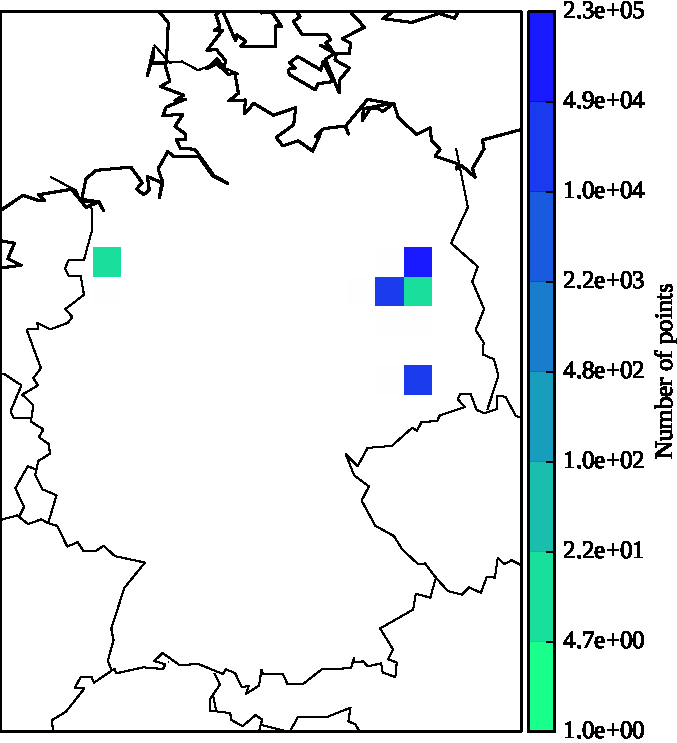
\includegraphics[width=\textwidth]{pix/freq_COM_ger_berlin.pdf}
		\caption{CM}
		%\label{fig:gull}
	\end{subfigure}
	%\,
	\begin{subfigure}[b]{.23\textwidth}
	\centering
	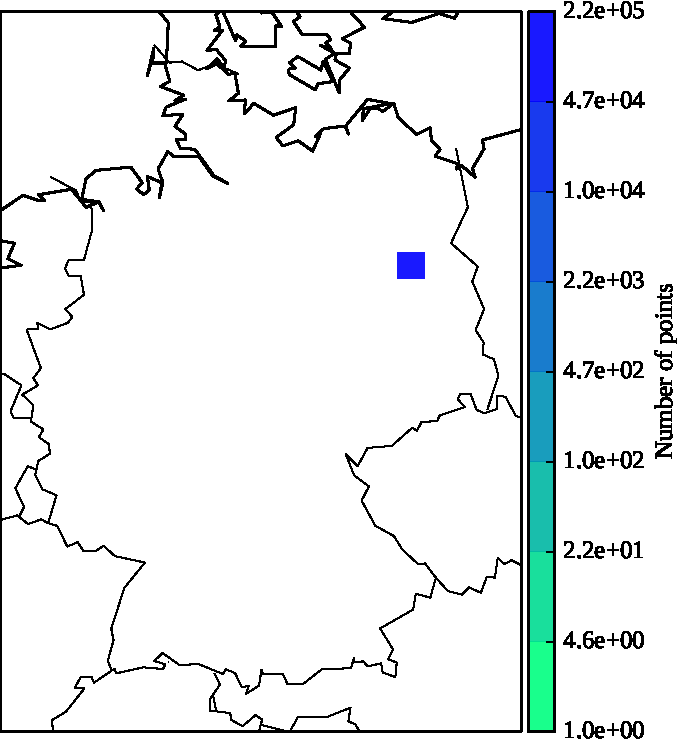
\includegraphics[width=\textwidth]{pix/freq_RW_ger_berlin.pdf}
		\caption{GM}
		%\label{fig:gull}
	\end{subfigure}
	\hfill
	\begin{subfigure}[b]{.23\textwidth}
	\centering
	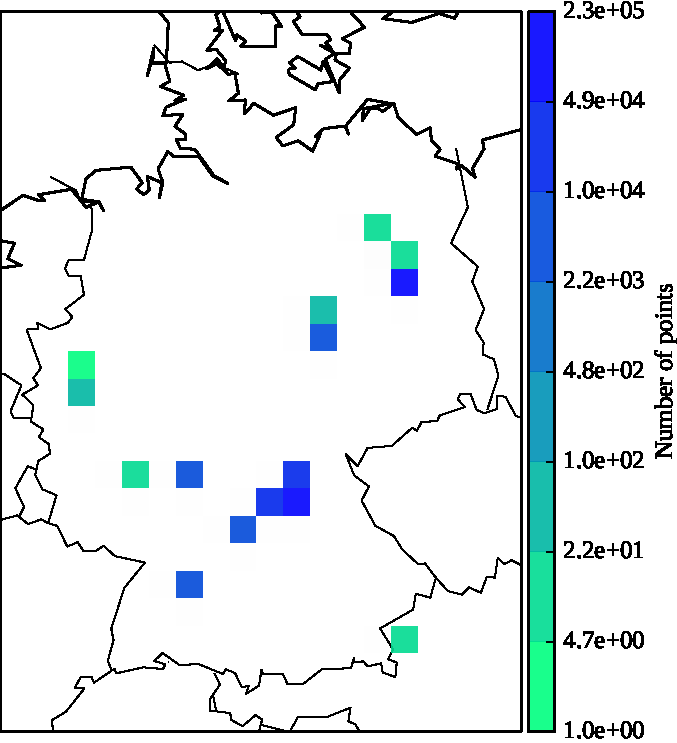
\includegraphics[width=\textwidth]{pix/freq_COM_ger_oster.pdf}
		\caption{CM}
		%\label{fig:gull}
	\end{subfigure}
	%\,
	\begin{subfigure}[b]{.23\textwidth}
	\centering
	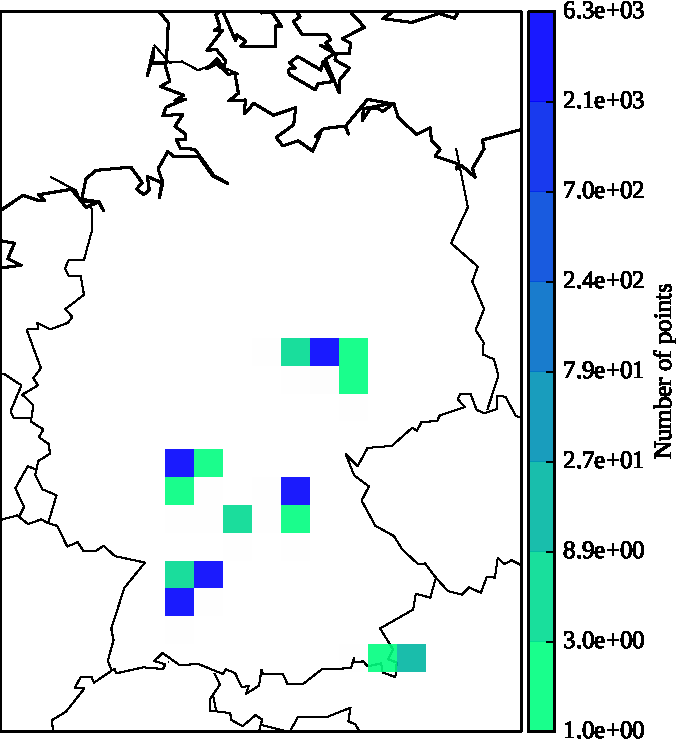
\includegraphics[width=\textwidth]{pix/freq_RW_ger_oster.pdf}
		\caption{GM}
		%\label{fig:gull}
	\end{subfigure}
	%
	\caption[Distributions for \emph{berlin}, \emph{oster} using dataset B.]{The left two distributions show $CM$ and $GM$ for \emph{berlin}, while the right pictures visualise the term \emph{oster} for dataset B.}
	\label{fig:B_comp}
\end{figure}

%                                     C USA
%
\newpage
\begin{center}
\captionof{table}{Statistics and used parameters for dataset C}
\small
\sisetup{table-parse-only}
\begin{tabular}{cSSSc}
\toprule
 & {clusters} &{clustered elements}&{noise}&{parameters}\\
\midrule
GM & 364 & 861138 & 225540&$km=300000, w_{text} = 0.1, \epsilon = 0.951$\\
CM & 343 & 1086024 & 654&$eps_{text} = 0.5, eps_{loc} = 7000$\\
\bottomrule
\end{tabular}
\end{center}
%
The last dataset C is Flickr data from the United States. The number of clusters are again very similar, but this time $GM$ has much noise, in contrast to the clusterings from dataset B. CQM scores (table~\ref{tbl:C_compare}) show a much better performance for $CM$ across the board with text and location distances alike. 
%
%
The terms used for this dataset are \emph{coast}, \emph{desert} and \emph{nature} because the same dataset as in \cite{Sengstock2012a} was used. Comparison pictures can be found in figure~\ref{fig:C_comp}. Distribution in space is similar between $GM$ and $CM$, but $CM$ has more more points in less spots, whereas $GM$ has more widespread distributions. Words describing the global region of America (\emph{unitedstates}, \emph{unitedstatesofamerica}, \emph{usa}) are unfortunately very common in all results and omitted in the further discussion.

\emph{coast} yields for $GM$ mostly cities or regions near to a coast, like \emph{houston}, \emph{california}, \emph{wortham}, \emph{sanfrancisco}, \emph{newyork} and \emph{vancuover}. General environmental terms (\emph{westcoast}, \emph{park}) appear less. Results for $CM$ are not as good, with the three top terms \emph{home45drumhillroad},\emph{elementsorganizer}, \emph{harrypotterparty} having nothing to do with a coast. Cities and environmental words are less frequent.

\enlargethispage{1\baselineskip}
\begin{table}[h]
\caption{CQM for dataset C}\label{tbl:C_compare}
\small
\centering
%\sisetup{table-parse-only}
\sisetup{table-format = 1.0(1)e2}
\begin{tabular}{cSSSS}
\toprule
Dataset & {DB} &{C}&{SW}&{D}\\
			& {\scriptsize $0<min<\infty$} &{\scriptsize $0<min<1$}&{\scriptsize $-1<max<1$}&{\scriptsize $0<max<\infty$}\\
\midrule
\multicolumn{5}{c}{Location distance}\\
\midrule
GM & 7.09e+00 & 7.01e-05 & 6.79e-01 & 2.17e-12\\
CM  & 6.96e-01 & 5.73e-07 & 8.78e-01 & 6.15e-04\\
R  & 1.29e+03 & 2.35e-01 & -1.41e-01 & 0.00e+00\\
\midrule
\multicolumn{5}{c}{Text distance}\\
\midrule
GM & 1.28e+00 & 2.70e-01 & 4.13e-01 & 0.00e+00\\
CM & 1.37e+00 & 1.42e-01 & 6.69e-01 & 0.00e+00\\
R & 3.90e+00 & 8.69e-01 & -2.05e-02 & 0.00e+00\\
\bottomrule
\end{tabular}
\end{table}

Mutual terms for \emph{desert} are \emph{nevada}, \emph{utah}, \emph{canyon} and \emph{water}, which is reasonable. $GM$ has among others more good words like \emph{mexico}, \emph{texas}, \emph{sierra},  \emph{arizona} and the global theme \emph{America} is not present. $CM$ has \emph{hike}, \emph{southwest}, \emph{desert} and \emph{rock}, but also unsuitable ones like \emph{chris} and \emph{deviatedseptum} (a common physical disorder of the nose). 

Unusual results are obtained with \emph{nature}. $CM$ shows again \emph{home45drumhillroad}, \emph{elementsorganizer}, \emph{harrypotterparty} as top results, with Microsoft Windows terms following (\emph{microsoft}, \emph{windows}, \emph{7}, \emph{skydrive}, \emph{live}) and the first \emph{nature} related term at position 26. $GM$ has more meaningful results: \emph{nature}, \emph{camping} and \emph{napavalley} are among the top ten terms, with \emph{sky}, \emph{park}, \emph{trees} and \emph{hiking} present after many different entries for \emph{tatoos} and \emph{tatto} studios.

\begin{figure}%[tbp]
	\begin{subfigure}[b]{.45\textwidth}
	\centering
	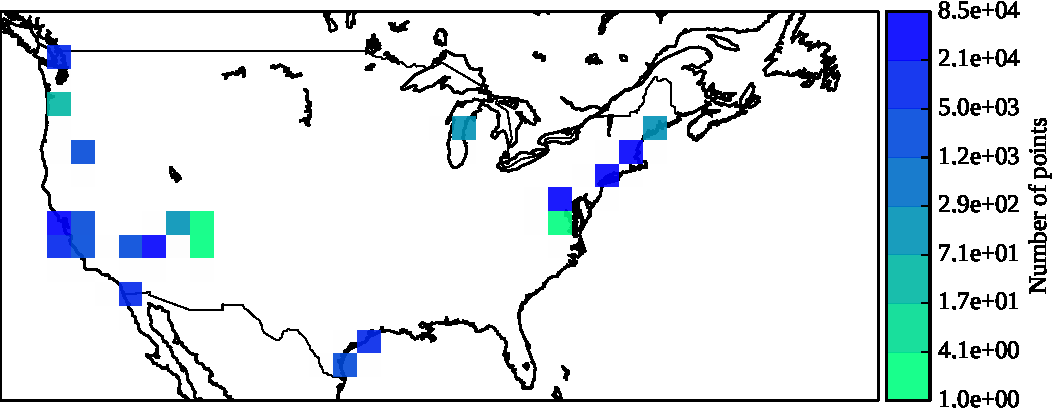
\includegraphics[width=\textwidth]{pix/freq_COM_usa_coast.pdf}
		%\caption{Frequency plot}
		%\label{fig:gull}
	\end{subfigure}
	\hfill
	\begin{subfigure}[b]{.45\textwidth}
	\centering
	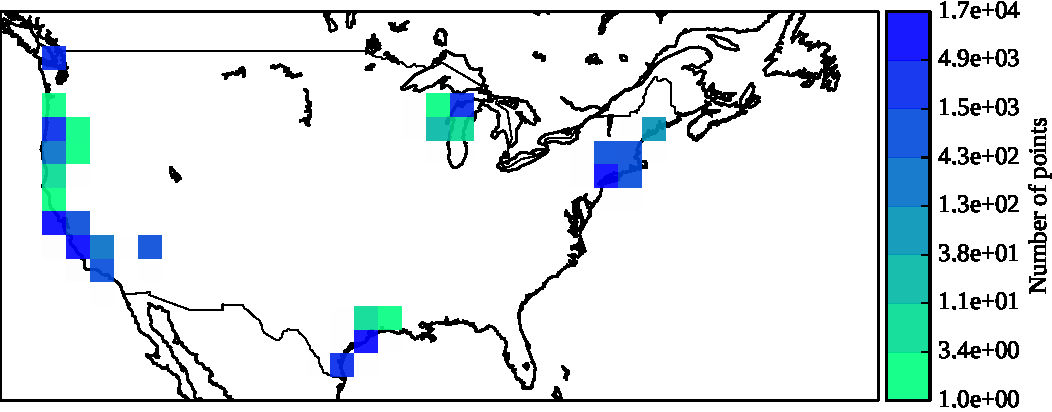
\includegraphics[width=\textwidth]{pix/freq_RW_usa_coast.pdf}
		%\caption{coast}
		%\label{fig:gull}
	\end{subfigure}
	\,
	\begin{subfigure}[b]{.45\textwidth}
	\centering
	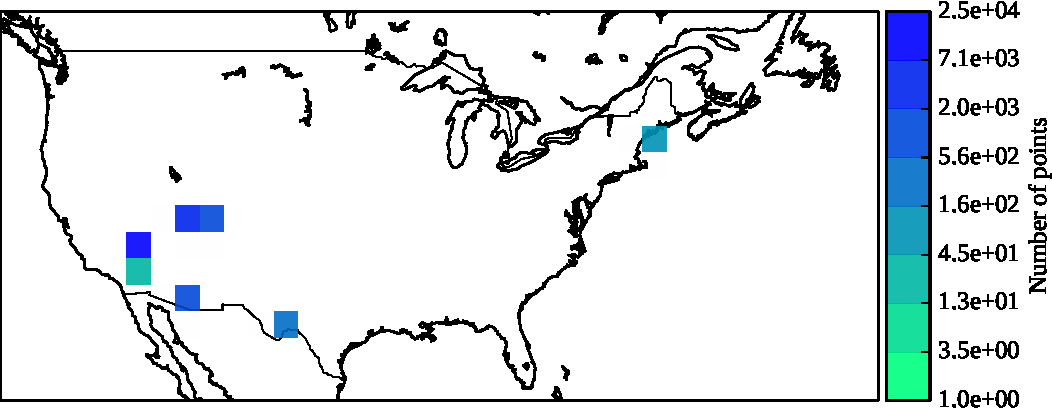
\includegraphics[width=\textwidth]{pix/freq_COM_usa_desert.pdf}
		%\caption{Frequency plot}
		%\label{fig:gull}
	\end{subfigure}
	\hfill
	\begin{subfigure}[b]{.45\textwidth}
	\centering
	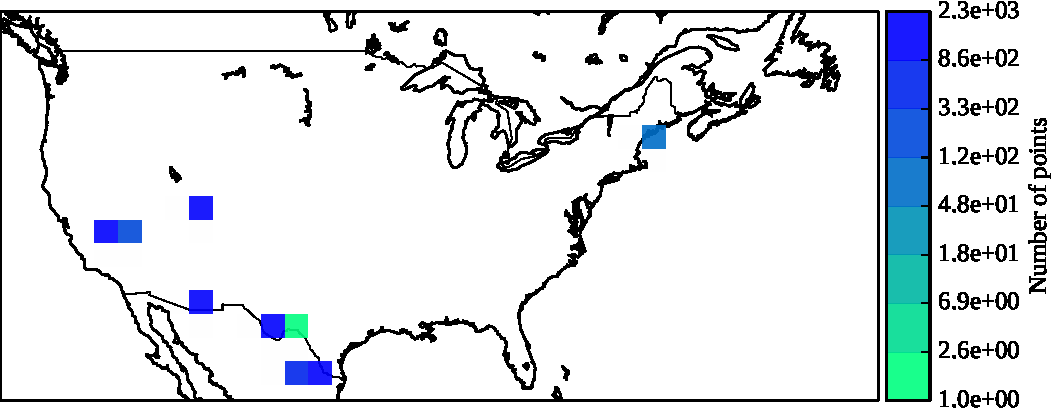
\includegraphics[width=\textwidth]{pix/freq_RW_usa_desert.pdf}
		%\caption{desert}
		%\label{fig:gull}
	\end{subfigure}
	\,
	\begin{subfigure}[b]{.45\textwidth}
	\centering
	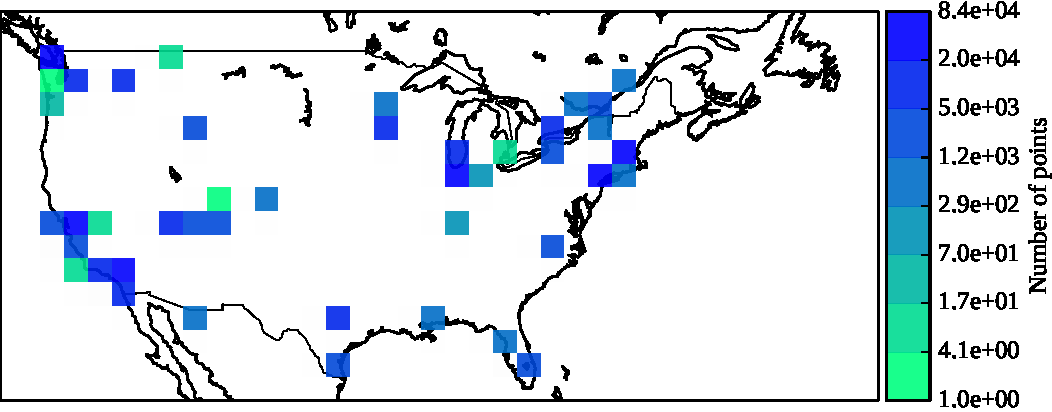
\includegraphics[width=\textwidth]{pix/freq_COM_usa_nature.pdf}
		\caption{CM}
		%\label{fig:gull}
	\end{subfigure}
	\hfill
	\begin{subfigure}[b]{.45\textwidth}
	\centering
	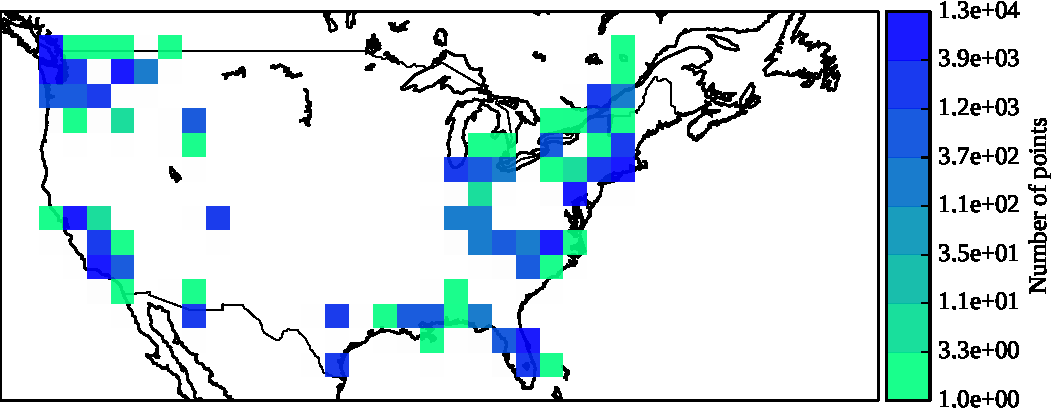
\includegraphics[width=\textwidth]{pix/freq_RW_usa_nature.pdf}
		\caption{GM}
		%\label{fig:gull}
	\end{subfigure}
	%
	\caption[Distributions for \emph{coast}, \emph{desert}, \emph{nature} with dataset C.]{The first column contains the plots for the combined metric and the second for the graph metric. The first row shows the distributions for \emph{coast}, the second for \emph{desert} and the third for \emph{nature}.}
	\label{fig:C_comp}
\end{figure}

\newpage
\noindent
$CM$ and $GM$ both deliver reasonable results, with $GM$ generally better geographic topics. Their performance is very dependent in the used dataset, as results for dataset A were poor compared to using datasets B or C.

These results were not exactly mirrored by the cluster quality measures. Compared to a random clustering, they show (some more, some less) if a clustering could generally be good. But directly comparing the scores, at least with the used basic distance functions, is not appropriate, as $CM$ usually has better scores, but $GM$ is qualitatively better. Using the jaccard distance for the CQMs resulted always in lower scores as using euclidean distance. The distance distribution with a majority of maximum distance and very few similarities seem to distort the ranges of the scores.

Despite the lack of comparability, the CQMs give generally good hints of the overall goodness of the results. Except the Dunn index ($D$) as presented in section~\ref{sec:cqm}, which in almost all cases has the same score of $0.0$, which leads to the assumption that real world cases have clusters in very near proximity more often than less. The Davies-Bouldin ($DB$) and $C$ indices fare quite well, but comparisons are always about the order of magnitude, and results are less constant in their representably of how well a result truly is. Silhouette width ($SW$) generates meaningful scores, which are easy to comprehend and correspond usually quite well to the observed characteristics of the clusterings.